\documentclass[12pt]{article}
\usepackage{setspace, graphicx, fullpage, amssymb, amsmath, epsfig, natbib, array, multirow, hyperref}
\usepackage{amsfonts, bm}
\usepackage{dcolumn}
\usepackage{subfigure, float}
\usepackage[margin=1in]{geometry}
\usepackage{verbatim}
\usepackage{url}
\usepackage{enumerate}
\newcolumntype{d}[1]{D{.}{.}{#1}}

\begin{document}

\begin{center}
\Large 08 February 2016
\end{center}

\section{Overview}

The main tasks I set out to accomplish over week as per our last meeting were as follows:

\begin{itemize}
	\item Check that we were sorting lopsided and close votes correctly

	\item Figure out who is being sorted as an extremist and not as complying to party calls

	\item Redo DV/IV regressions with both IVs by party and majority/minority status

	\item Test adding different levels of randomness to the initial lopsided/close vote seeding
\end{itemize}

\noindent
After checking the first item, I worked on the others. I include the plots and tables most relevant to these below.

Over the course of this week, I continued digging into the old functions and comparing them with the new functions. I found four differences which I had previously missed. The first of these I discussed with you through email. We had moved to allowing the function to stop not only when the number of switched votes dropped below a certain threshold, but also when the number of switched votes began rising again. This is in line with the 2013 paper. Having run the algorithm with our new stopping rule, I find it to have only a negligible impact on vote sorting. Summary tables for this sorting are included.

The second through fourth, I found later in the week and thus saved for the update. None of them seem promising. The first is that we have begun dropping votes which had 4 or fewer Senators on one side. I was unable to find anything which mentioned their exclusion or inclusion in the 2013 paper or its appendices, so I looked into them. Running a single iteration of the sorting function manually initially led to more party calls than a counterpart without them, but running the algorithm all the way through proved to lead to a much larger increase in noncalls. Additionally, in the previous Senate Party Calls we were sorting votes by OLS rather than a bias-reduced logit and had party line votes dropped rather than coded as definite party calls. The first of these leads the current algorithm to be more like the one used for the 2013 paper and the second makes sense theoretically and could not possibly be driving the differences we are seeing.





\section{Tables and Figures}

\subsection{Digging into p < 0.05 Party Call Coding}

I first show plots in which characteristics I thought likely to go along with non-responsiveness are broken down by party. I do this by providing plots with separate colors for points based on the value in that area, with separate Loess curves fitted to each category. I found that the switch in responsiveness seems to happen around the ideological extremism value of 1 for both Democrats and Republicans and so I provide tables of MCs who are above this threshold and non-responsive to party calls. Finally, I conducted regression analysis with party call responsiveness as the DV and noncall response and extremism as IVs.

\begin{figure}[h]
	\caption{Main DV and Ideological Extremism - Majority and Minority Party Democrats \textit{Note}: The light gray line and dots are for Congress 107.}
	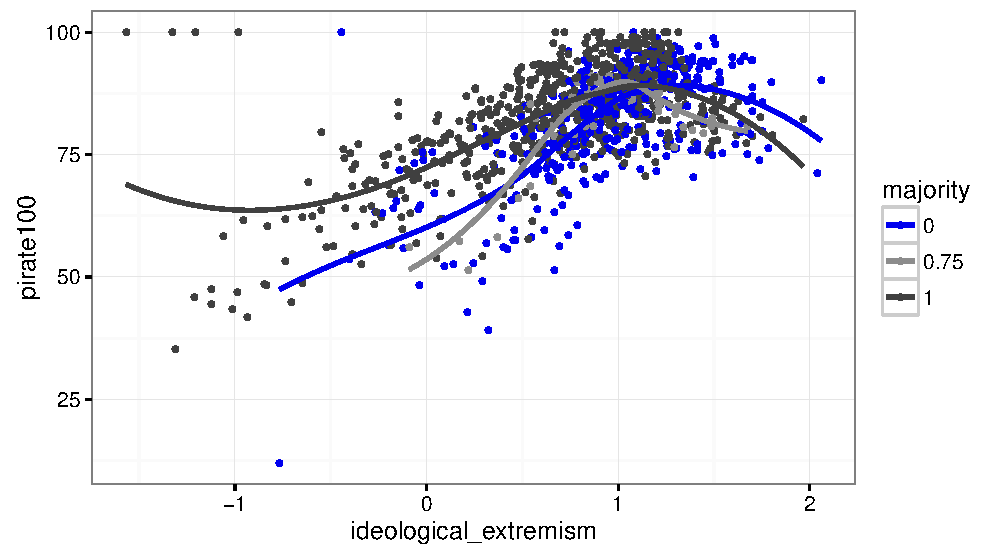
\includegraphics[width = \textwidth]{C:/Users/Ethan/Documents/GitHub/partycalls/plots/senate_p_05_dem_iv-dv_2_majority.pdf}
\end{figure}

\begin{figure}[h]
	\caption{Main DV and Ideological Extremism - Southern and Other Democrats}
	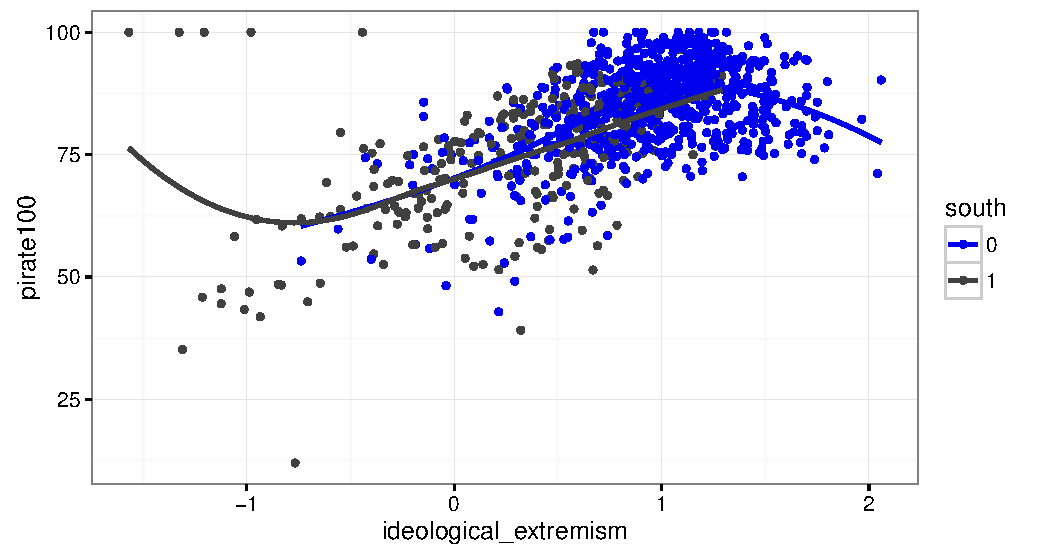
\includegraphics[width = \textwidth]{C:/Users/Ethan/Documents/GitHub/partycalls/plots/senate_p_05_dem_iv-dv_2_south.pdf}
\end{figure}

\begin{figure}[h]
	\caption{Main DV and Ideological Extremism - Majority and Minority Party Republicans \textit{Note}: The light gray line and dots are for Congress 107.}
	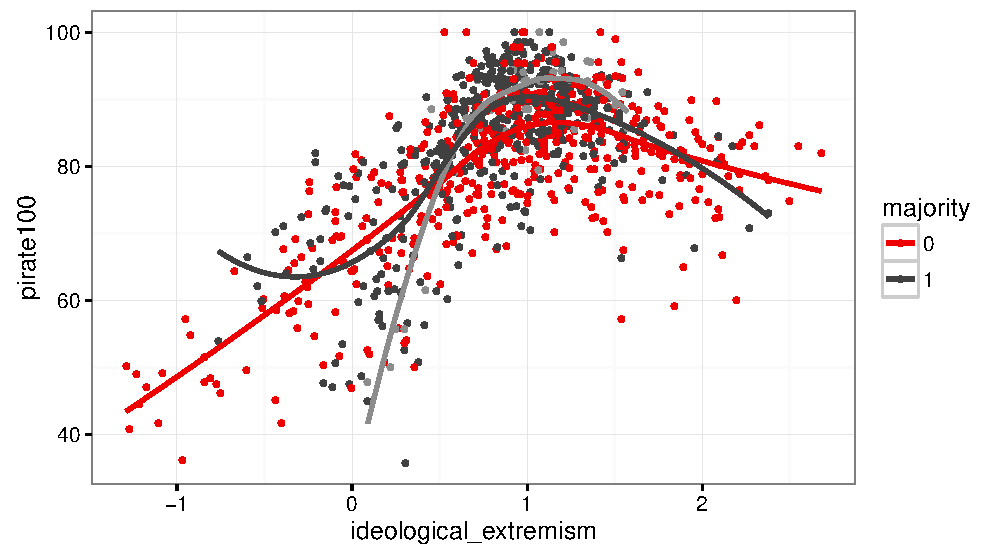
\includegraphics[width = \textwidth]{C:/Users/Ethan/Documents/GitHub/partycalls/plots/senate_p_05_rep_iv-dv_2_majority.pdf}
\end{figure}

\begin{figure}[h]
	\caption{Main DV and Ideological Extremism - Southern and Other Republicans}
	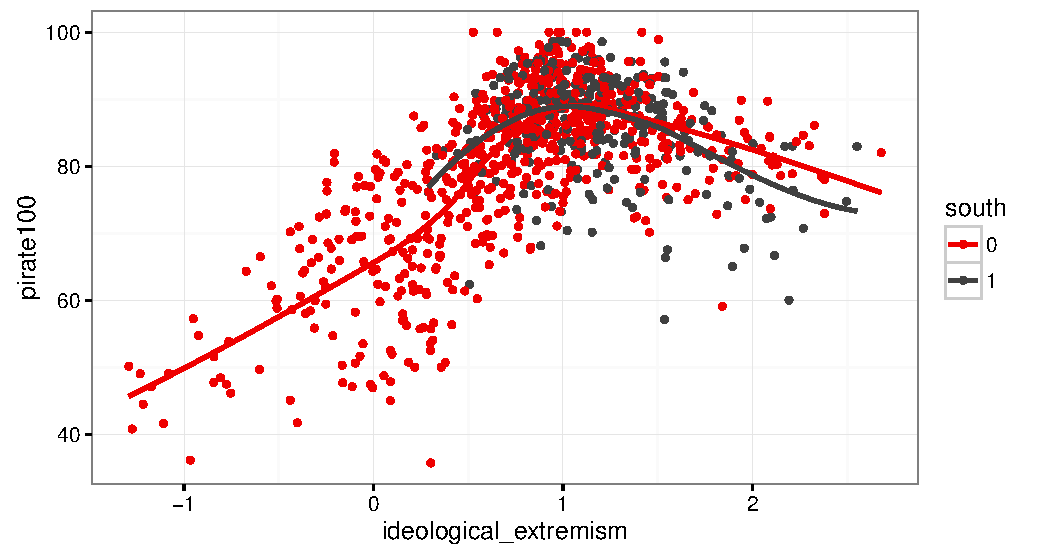
\includegraphics[width = \textwidth]{C:/Users/Ethan/Documents/GitHub/partycalls/plots/senate_p_05_rep_iv-dv_2_south.pdf}
\end{figure}

\begin{figure}[h]
	\caption{Main DV and Ideological Extremism - Gingrich Senators and Other Republicans}
	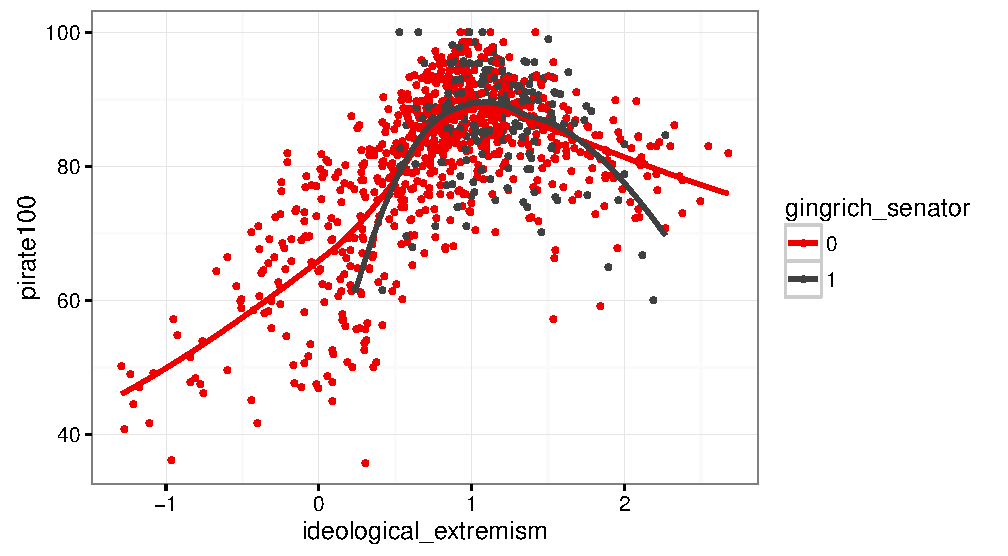
\includegraphics[width = \textwidth]{C:/Users/Ethan/Documents/GitHub/partycalls/plots/senate_p_05_rep_iv-dv_2_gingrich.pdf}
 \end{figure}

% latex table generated in R 3.3.2 by xtable 1.8-2 package
% Sun Feb 05 15:06:25 2017
\begin{table}[ht]
	\centering
		\caption{Democrats With Extremism $ \textgreater $ 1 and Party Call Response $ \textless $ 75\%}
	\begin{tabular}{rlrrrrr}
		\hline
		congress & mc & votes & pres vote & extremism & pfrate100 & pirate100 \\
		\hline
		95 & ABOUREZK (D SD) & 642 & 0.49 & 1.14 & 70.56 & 70.55 \\
		96 & LEAHY (D VT) & 972 & 0.44 & 1.00 & 86.56 & 74.76 \\
		97 & RANDOLPH (D WV) & 964 & 0.52 & 1.02 & 85.06 & 72.58 \\
		97 & WILLIAMS (D NJ) & 443 & 0.43 & 1.20 & 84.57 & 71.67 \\
		97 & KENNEDY (D MA) & 880 & 0.50 & 2.04 & 82.68 & 71.12 \\
		97 & PELL (D RI) & 951 & 0.56 & 1.12 & 77.89 & 72.11 \\
		97 & CRANSTON (D CA) & 873 & 0.41 & 1.49 & 79.21 & 74.81 \\
		97 & METZENBAUM (D OH) & 883 & 0.44 & 1.74 & 85.37 & 73.96 \\
		97 & TSONGAS (D MA) & 865 & 0.50 & 1.39 & 78.63 & 70.44 \\
		97 & BRADLEY (D NJ) & 917 & 0.43 & 1.25 & 82.76 & 74.65 \\
		101 & BIDEN (D DE) & 626 & 0.44 & 1.03 & 79.17 & 73.29 \\
		101 & BRADLEY (D NJ) & 625 & 0.43 & 1.19 & 75.73 & 73.46 \\
		\hline
	\end{tabular}
\end{table}

% latex table generated in R 3.3.2 by xtable 1.8-2 package
% Sun Feb 05 15:09:49 2017
\begin{table}[ht]
	\centering
	\caption{Republicans With Extremism $ \textgreater $ 1 and Party Call Response $ \textless $ 75\%}
	\begin{tabular}{rlrrrrr}
		\hline
		congress & mc & votes cast & pres vote & extremism & pfrate100 & pirate100 \\
		\hline
		93 & GOLDWATER (R AZ) & 788 & 0.67 & 1.81 & 73.70 & 72.83 \\
		93 & MCCLURE (R ID) & 967 & 0.71 & 1.38 & 76.39 & 72.28 \\
		93 & SCOTT (R VA) & 1000 & 0.69 & 1.55 & 69.64 & 67.52 \\
		93 & HELMS (R NC) & 1083 & 0.71 & 2.10 & 72.10 & 72.42 \\
		94 & GOLDWATER (R AZ) & 804 & 0.67 & 2.09 & 69.56 & 73.64 \\
		94 & SCOTT (R VA) & 1153 & 0.69 & 1.87 & 64.01 & 74.07 \\
		94 & HELMS (R NC) & 1276 & 0.71 & 2.04 & 65.90 & 74.62 \\
		95 & YOUNG (R ND) & 935 & 0.53 & 1.00 & 85.69 & 74.55 \\
		98 & SYMMS (R ID) & 615 & 0.73 & 2.38 & 70.79 & 72.95 \\
		98 & HELMS (R NC) & 648 & 0.51 & 1.96 & 70.49 & 67.76 \\
		98 & EAST (R NC) & 624 & 0.51 & 2.27 & 69.13 & 70.73 \\
		98 & NICKLES (R OK) & 646 & 0.63 & 1.54 & 74.26 & 66.36 \\
		99 & NICKLES (R OK) & 739 & 0.69 & 1.02 & 83.08 & 70.40 \\
		100 & HELMS (R NC) & 737 & 0.62 & 2.50 & 68.29 & 74.77 \\
		101 & HELMS (R NC) & 633 & 0.58 & 2.07 & 74.92 & 72.22 \\
		101 & HUMPHREY (R NH) & 615 & 0.63 & 1.44 & 75.74 & 71.88 \\
		110 & BUNNING (R KY) & 636 & 0.60 & 1.37 & 85.98 & 73.85 \\
		110 & KYL (R AZ) & 644 & 0.55 & 1.46 & 83.99 & 70.15 \\
		110 & COBURN (R OK) & 607 & 0.66 & 1.90 & 81.08 & 65.00 \\
		110 & VITTER (R LA) & 628 & 0.57 & 1.34 & 87.32 & 74.63 \\
		110 & DEMINT (R SC) & 634 & 0.59 & 2.12 & 82.44 & 66.67 \\
		110 & SESSIONS (R AL) & 643 & 0.63 & 1.15 & 88.37 & 70.15 \\
		110 & ENZI (R WY) & 636 & 0.70 & 1.39 & 87.62 & 72.46 \\
		112 & DEMINT (R SC) & 431 & 0.55 & 2.19 & 77.96 & 60.00 \\
		112 & PAUL (R KY) & 462 & 0.58 & 1.54 & 74.46 & 57.14 \\
		112 & LEE (R UT) & 472 & 0.65 & 1.84 & 76.15 & 59.09 \\
		\hline
	\end{tabular}
\end{table}

\begin{table}
	\begin{center}
		\caption{Main DV and IV Regressions}
		\begin{tabular}{l c c c c }
			\hline
			& Democrats & Republicans & Majority & Minority \\
			\hline
			pfrate100              & $0.879^{***}$ & $0.847^{***}$  & $0.895^{***}$ & $0.777^{***}$  \\
			& $(0.028)$     & $(0.026)$      & $(0.026)$     & $(0.030)$      \\
			ideological\_extremism & $0.810$       & $2.350^{***}$  & $1.442^{**}$  & $2.471^{***}$  \\
			& $(0.527)$     & $(0.444)$      & $(0.481)$     & $(0.529)$      \\
			(Intercept)            & $7.695^{***}$ & $10.332^{***}$ & $6.442^{**}$  & $15.341^{***}$ \\
			& $(2.098)$     & $(1.955)$      & $(2.026)$     & $(2.192)$      \\
			\hline
			R$^2$                  & 0.666         & 0.669          & 0.694         & 0.631          \\
			Adj. R$^2$             & 0.665         & 0.668          & 0.694         & 0.630          \\
			Num. obs.              & 1039          & 951            & 1049          & 843            \\
			RMSE                   & 6.433         & 6.758          & 6.093         & 7.120          \\
			\hline
			\multicolumn{5}{l}{\scriptsize{$^{***}p<0.001$, $^{**}p<0.01$, $^*p<0.05$}}
		\end{tabular}
	\end{center}
\end{table}

\clearpage

\subsection{Senate Vote Coding With Semi-Random Initial Noncalls}

In order to test a combination of first round noncalls being selected by lopsided or close votes and random chance I added a model parameter which can randomly switch a certain percent of the close and lopsided votes. In order to test this, I ran the algorithm with 25, 50, and 75 percent of these switched as well as one with all selected at random. Of these, the 50\% would be the most similar in its parameters to random selection and the 75\% is like reverse selection with a 25\% switch. These otherwise matched the current sorting algorithm we have been using (with the agreed upon $ p < 0.05 $ threshold). These performed roughly the same as one another, showing that our initial selection has little to no influence on the performance of the sorting function.

% latex table generated in R 3.3.2 by xtable 1.8-2 package
% Mon Feb 06 11:51:36 2017
\begin{table}[ht]
	\centering
	\caption{Senate Coding with 25\% of Votes Initially Switched by Congress}
	\begin{tabular}{rrrr}
		\hline
		congress & party calls & noncalls & gray votes \\
		\hline
		93 & 350 & 590 &   4 \\
		94 & 407 & 689 &   0 \\
		95 & 277 & 710 &   2 \\
		96 & 348 & 535 &   3 \\
		97 & 322 & 424 &  30 \\
		98 & 216 & 316 &   8 \\
		99 & 186 & 445 &   5 \\
		100 & 213 & 378 &  13 \\
		101 & 162 & 322 &   4 \\
		102 & 132 & 323 &   5 \\
		103 & 135 & 473 &  13 \\
		104 & 157 & 598 &  36 \\
		105 &  89 & 365 &  12 \\
		106 & 110 & 394 &  10 \\
		107 &  69 & 367 &   7 \\
		108 &  70 & 418 &  11 \\
		109 &  87 & 414 &   5 \\
		110 &  71 & 442 &  10 \\
		111 &  94 & 499 &  12 \\
		112 &  44 & 344 &   4 \\
		\hline
		Total: & 3539 & 9046 & 194 \\
		Mean: & 177.0 & 452.3 & 9.7 \\
		sd: & 109.9 & 117.8 & 8.9 \\
		\hline
	\end{tabular}
\end{table}

% latex table generated in R 3.3.2 by xtable 1.8-2 package
% Mon Feb 06 12:02:07 2017
\begin{table}[ht]
	\centering
		\caption{Senate Coding with 25\% of Votes Initially Switched by Lopsided/Close}
	\begin{tabular}{rrrr}
		\hline
		& party call  & noncall & gray \\
		\hline
		Lopsided & 1397 & 4180 & 109 \\
		Close & 2142 & 4866 & 85 \\
		\hline
	\end{tabular}
\end{table}

% latex table generated in R 3.3.2 by xtable 1.8-2 package
% Mon Feb 06 12:07:34 2017
\begin{table}[ht]
	\centering
	\caption{Senate Coding with 50\% of Votes Initially Switched by Congress}
	\begin{tabular}{rrrr}
		\hline
		congress & party calls & noncalls & gray votes \\
		\hline
		93 & 350 & 590 &   4 \\
		94 & 407 & 689 &   0 \\
		95 & 277 & 710 &   2 \\
		96 & 348 & 535 &   3 \\
		97 & 323 & 423 &  30 \\
		98 & 219 & 315 &   6 \\
		99 & 184 & 441 &  11 \\
		100 & 212 & 378 &  14 \\
		101 & 160 & 324 &   4 \\
		102 & 131 & 325 &   4 \\
		103 & 136 & 474 &  11 \\
		104 & 158 & 605 &  28 \\
		105 &  90 & 364 &  12 \\
		106 & 109 & 393 &  12 \\
		107 &  69 & 367 &   7 \\
		108 &  72 & 418 &   9 \\
		109 &  87 & 414 &   5 \\
		110 &  71 & 444 &   8 \\
		111 &  92 & 500 &  13 \\
		112 &  42 & 346 &   4 \\
		\hline
		Total: & 3537 & 9055 & 187 \\
		Mean: & 176.9 & 452.8 & 9.4 \\
		sd: & 110.2 & 118.1 & 7.8 \\
		\hline
	\end{tabular}
\end{table}

% latex table generated in R 3.3.2 by xtable 1.8-2 package
% Mon Feb 06 12:02:07 2017
\begin{table}[ht]
	\centering
	\caption{Senate Coding with 50\% of Votes Initially Switched by Lopsided/Close}
	\begin{tabular}{rrrr}
		\hline
		& party call  & noncall & gray \\
		\hline
		Lopsided & 1398 & 4179 & 109 \\
		Close & 2139 & 4876 & 78 \\
		\hline
	\end{tabular}
\end{table}

% latex table generated in R 3.3.2 by xtable 1.8-2 package
% Mon Feb 06 12:15:23 2017
\begin{table}[ht]
	\centering
	\caption{Senate Coding with 75\% of Votes Initially Switched by Congress}
	\begin{tabular}{rrrr}
		\hline
		congress & party calls & noncalls & gray votes \\
		\hline
		93 & 350 & 590 &   4 \\
		94 & 407 & 689 &   0 \\
		95 & 277 & 710 &   2 \\
		96 & 348 & 535 &   3 \\
		97 & 336 & 429 &  11 \\
		98 & 217 & 322 &   1 \\
		99 & 185 & 444 &   7 \\
		100 & 212 & 376 &  16 \\
		101 & 160 & 324 &   4 \\
		102 & 132 & 324 &   4 \\
		103 & 129 & 468 &  24 \\
		104 & 158 & 604 &  29 \\
		105 &  89 & 365 &  12 \\
		106 & 109 & 391 &  14 \\
		107 &  67 & 367 &   9 \\
		108 &  71 & 419 &   9 \\
		109 &  86 & 415 &   5 \\
		110 &  71 & 441 &  11 \\
		111 &  93 & 499 &  13 \\
		112 &  42 & 346 &   4 \\
		\hline
		Total: & 3539 & 9058 & 182 \\
		Mean: & 177.0 & 452.9 & 9.1 \\
		sd: & 111.4 & 117.6 & 7.5 \\
		\hline
	\end{tabular}
\end{table}

% latex table generated in R 3.3.2 by xtable 1.8-2 package
% Mon Feb 06 12:02:07 2017
\begin{table}[ht]
	\centering
	\caption{Senate Coding with 75\% of Votes Initially Switched by Lopsided/Close}
	\begin{tabular}{rrrr}
		\hline
		& party call  & noncall & gray \\
		\hline
		Lopsided & 1418 & 4177 & 91 \\
		Close & 2121 & 4881 & 91 \\
		\hline
	\end{tabular}
\end{table}


% latex table generated in R 3.3.2 by xtable 1.8-2 package
% Mon Feb 06 12:25:47 2017
\begin{table}[ht]
	\centering
	\caption{Senate Coding with 75\% of Votes Initially Sorted Randomly by Congress}
	\begin{tabular}{rrrr}
		\hline
		congress & party calls & noncalls & gray votes \\
		\hline
		93 & 350 & 590 &   4 \\
		94 & 407 & 689 &   0 \\
		95 & 277 & 709 &   3 \\
		96 & 348 & 535 &   3 \\
		97 & 321 & 424 &  31 \\
		98 & 218 & 312 &  10 \\
		99 & 185 & 442 &   9 \\
		100 & 213 & 376 &  15 \\
		101 & 154 & 327 &   7 \\
		102 & 132 & 322 &   6 \\
		103 & 137 & 474 &  10 \\
		104 & 158 & 604 &  29 \\
		105 &  90 & 365 &  11 \\
		106 & 106 & 391 &  17 \\
		107 &  69 & 367 &   7 \\
		108 &  71 & 416 &  12 \\
		109 &  87 & 414 &   5 \\
		110 &  74 & 439 &  10 \\
		111 &  94 & 499 &  12 \\
		112 &  42 & 346 &   4 \\
		\hline
		Total: & 3533 & 9041 & 205 \\
		Mean: & 176.7 & 452.0 & 10.3 \\
		sd: & 110.0 & 118.2 & 8.0 \\
		\hline
	\end{tabular}
\end{table}

% latex table generated in R 3.3.2 by xtable 1.8-2 package
% Mon Feb 06 12:02:07 2017
\begin{table}[ht]
	\centering
	\caption{Senate Coding with Votes Initially Sorted Randomly by Lopsided/Close}
	\begin{tabular}{rrrr}
		\hline
		& party call  & noncall & gray \\
		\hline
		Lopsided & 1403 & 4167 & 116 \\
		Close & 2130 & 4874 & 89 \\
		\hline
	\end{tabular}
\end{table}

\clearpage

\subsection{Senate Vote Coding Other Tests}

In this section I provide tables for the vote coding provided by different stopping rules and inclusion of very lopsided votes. The first of these, much like different selection of initial noncalls, has little influence on the vote sorting. The second Gives us many more noncalls while having little impact on the number of party calls.

% latex table generated in R 3.3.2 by xtable 1.8-2 package
% Mon Feb 06 13:00:07 2017
\begin{table}[ht]
	\centering
	\caption{Senate Vote Sorting by Congress, 1\% Vote Switch Stopping Rule}
	\begin{tabular}{rrrr}
		\hline
		congress & party calls & noncalls & gray votes \\
		\hline
		93 & 350 & 590 &   4 \\
		94 & 407 & 688 &   1 \\
		95 & 278 & 709 &   2 \\
		96 & 348 & 535 &   3 \\
		97 & 336 & 428 &  12 \\
		98 & 225 & 310 &   5 \\
		99 & 186 & 445 &   5 \\
		100 & 235 & 363 &   6 \\
		101 & 164 & 318 &   6 \\
		102 & 132 & 324 &   4 \\
		103 & 136 & 472 &  13 \\
		104 & 158 & 606 &  27 \\
		105 &  89 & 364 &  13 \\
		106 & 109 & 394 &  11 \\
		107 &  69 & 367 &   7 \\
		108 &  71 & 418 &  10 \\
		109 &  86 & 414 &   6 \\
		110 &  73 & 443 &   7 \\
		111 &  94 & 499 &  12 \\
		112 &  44 & 344 &   4 \\
		\hline
		Total: & 3590 & 9031 & 158 \\
		Mean: & 179.5 & 451.6 & 7.9 \\
		sd: & 111.5 & 119.1 & 5.8 \\
		\hline
	\end{tabular}
\end{table}

% latex table generated in R 3.3.2 by xtable 1.8-2 package
% Mon Feb 06 12:02:07 2017
\begin{table}[ht]
	\centering
	\caption{Senate Vote Sorting by Lopsided/Close, 1\% Vote Switch Stopping Rule}
	\begin{tabular}{rrrr}
		\hline
		& party call  & noncall & gray \\
		\hline
		Lopsided & 1397 & 4180 & 109 \\
		Close & 2142 & 4866 & 85 \\
		\hline
	\end{tabular}
\end{table}


% latex table generated in R 3.3.2 by xtable 1.8-2 package
% Mon Feb 06 13:12:37 2017
\begin{table}[ht]
	\centering
	\caption{Senate Vote Sorting by Congress, 0.5\% Vote Switch Stopping Rule}
		\begin{tabular}{rrrr}
		\hline
		congress & party calls & noncalls & gray votes \\
		\hline
		93 & 350 & 590 &   4 \\
		94 & 407 & 688 &   1 \\
		95 & 277 & 709 &   3 \\
		96 & 348 & 535 &   3 \\
		97 & 318 & 420 &  38 \\
		98 & 224 & 311 &   5 \\
		99 & 185 & 441 &  10 \\
		100 & 236 & 363 &   5 \\
		101 & 165 & 318 &   5 \\
		102 & 132 & 324 &   4 \\
		103 & 135 & 473 &  13 \\
		104 & 158 & 605 &  28 \\
		105 &  89 & 365 &  12 \\
		106 & 109 & 392 &  13 \\
		107 &  69 & 367 &   7 \\
		108 &  71 & 418 &  10 \\
		109 &  87 & 414 &   5 \\
		110 &  71 & 444 &   8 \\
		111 &  94 & 499 &  12 \\
		112 &  43 & 344 &   5 \\
		\hline
		Total: & 3568 & 9020 & 191 \\
		Mean: & 178.4 & 451 & 9.6 \\
		sd: & 110.4 & 119.1 & 8.9 \\
		\hline
	\end{tabular}
\end{table}

% latex table generated in R 3.3.2 by xtable 1.8-2 package
% Mon Feb 06 12:02:07 2017
\begin{table}[ht]
	\centering
	\caption{Senate Vote Sorting by Lopsided/Close, 0.5\% Vote Switch Stopping Rule}
	\begin{tabular}{rrrr}
		\hline
		& party call  & noncall & gray \\
		\hline
		Lopsided & 1395 & 4187 & 104 \\
		Close & 2173 & 4833 & 87 \\
		\hline
	\end{tabular}
\end{table}

% latex table generated in R 3.3.2 by xtable 1.8-2 package
% Mon Feb 06 13:24:33 2017
\begin{table}[ht]
	\centering
	\caption{Senate Vote Sorting by Congress, Keep Very Lopsided Votes in Analysis}
	\begin{tabular}{rrrr}
		\hline
		congress & party\_call\_count & noncall\_count & gray\_vote\_count \\
		\hline
		93 & 356 & 779 &   3 \\
		94 & 409 & 902 &   0 \\
		95 & 278 & 876 &   2 \\
		96 & 346 & 704 &   4 \\
		97 & 324 & 553 &  89 \\
		98 & 228 & 432 &   3 \\
		99 & 176 & 526 &  38 \\
		100 & 238 & 548 &  13 \\
		101 & 171 & 461 &   6 \\
		102 & 133 & 408 &   9 \\
		103 & 145 & 559 &  20 \\
		104 & 165 & 720 &  34 \\
		105 &  99 & 508 &   5 \\
		106 & 117 & 540 &  15 \\
		107 &  77 & 552 &   4 \\
		108 &  79 & 585 &  11 \\
		109 &  91 & 550 &   4 \\
		110 &  78 & 574 &   5 \\
		111 & 105 & 583 &   8 \\
		112 &  47 & 436 &   3 \\
		\hline
		Total: & 3662 & 11796 & 276 \\
		Mean: & 183.1 & 589.8 & 13.8 \\
		sd: & 108.5 & 138.4 & 20.4 \\
		\hline
	\end{tabular}
\end{table}

% latex table generated in R 3.3.2 by xtable 1.8-2 package
% Mon Feb 06 12:02:07 2017
\begin{table}[ht]
	\centering
	\caption{Senate Vote Sorting by Lopsided/Close, Keep Very Lopsided Votes in Analysis}
	\begin{tabular}{rrrr}
		\hline
		& party call  & noncall & gray \\
		\hline
		Lopsided & 1476 & 7048 & 116 \\
		Close & 2186 & 4748 & 160 \\
		\hline
	\end{tabular}
\end{table}











\end{document}
